\documentclass[11pt]{article}

\usepackage[letterpaper,left=1.6in,right=1.6in,top=1.2in,bottom=1.2in]{geometry}

\usepackage[T1]{fontenc}
\usepackage[utf8]{inputenc}

\usepackage{lmodern}
\usepackage{amssymb,amsmath}
\usepackage{graphicx}
\usepackage[11pt]{moresize}

\setcounter{secnumdepth}{0}

%\usepackage[vlined]{algorithm2e}
\usepackage{algorithm,algorithmic}
\usepackage{paralist}
\usepackage{tikz}
\usepackage{xcolor,colortbl}

\begin{document}
\begin{center}
\begin{HUGE}{\bf A6 - Shipping Game}\\ \end{HUGE}
\vspace{10mm}
\begin{LARGE} Contents\\ \end{LARGE}
\noindent\rule{8cm}{0.4pt}
\begin{enumerate} \begin{large}
\item Game Overview
\item Installation
\item Class Explanation
\item Your Tasks
\item Competition
\end{large}\end{enumerate}
\end{center}
\newpage

\section{1. Game Overview}
In Shipping Game (less descriptive name pending) you play the part of a shipping company engineer who makes sure that deliveries get where they're going in a timely fashion. In an instance of Shipping Game, you are presented with an undirected, weighted graph that represents the world. The nodes in this graph are cities where parcels are picked up from or dropped off to, and the edges are highways that connect the cities. Parcels are distributed around the map, each with a starting location (a city in the map) and a delivery destination (a different city in the map).\\
\centerline{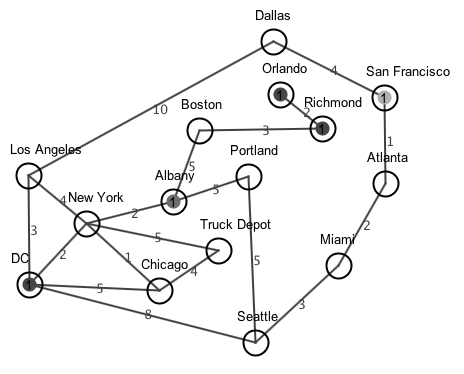
\includegraphics[scale=0.8]{map1.png}}\\
Cities in the map are labeled with their name, highways with their length. The smaller filled-in circles that appear in some cities are parcels that need to be picked up and delivered elsewhere on the map.\\

In order to accomplish this task, you have a fleet of trucks that you are able to control. At the beginning of the game you have the option to give your trucks instructions. Additionally, whenever a truck reaches an important point, such as reaching its destination after traveling a highway, it will let you know so you can give it additional instruction. All Trucks begin the game on the Truck Depot city (there will be exactly one truck depot in every map) and must return there after delivering all parcels for the game to end.

\newpage
\section{2. Installation}
Nerrrr....

\newpage
\section{3. Class Explanation}
sadf

\newpage
\section{4. Your Tasks}
In order to complete the assignment, your primary task is write a class extending the abstract Manager class explained in the previous section. In order to do this, you will have to override and implement the two abstract methods declared in the Manager class: \textbf{run()} and \textbf{truckNotification(Truck t, Notification message)}. These two methods determine the behavior of the trucks in the game.\\

run() is called by the game as soon as the game begins, and allows you to do initial computation and give your trucks their initial set of instructions. Additionally, the body of run() will run in a separate thread from all of the trucks, so you can continue to do computation after the trucks have begun their travel. Your implementation can either loop forever and continually add information to the trucks or execute a single time for initial instructions and then rely on the truckNotification method for further interaction.\\

truckNotification(Truck t, Notification message) is called by trucks whenever they do something of note. For a full list of the reasons why a truck would call this method, see Manager.Notification in the previous section and in the javadoc. This method is called by the truck in its own thread in order to ask for more instructions. For example, upon arrival at a new node in the graph, the truck may send a notification that there is at least one parcel at the current node. Perhaps you want that truck to pick up that parcel before continuing on its route.


\end{document}